% ---------------------------------------------------------------------------
% Пример главы / Example chapter.
%
% Каждая глава --- отдельная папка Dissertation/partN/ с файлом partN.tex и
% папкой pictures/ для изображений. Глава подключается из dissertation.tex
% командой \subimport{Dissertation/partN/}{partN}, поэтому рисунки можно
% подключать как \includegraphics{pictures/...}.
%
% Each chapter lives in its own folder Dissertation/partN/ with a partN.tex file
% and a pictures/ subfolder. It is pulled in from dissertation.tex with
% \subimport{Dissertation/partN/}{partN}, so figures are included as
% \includegraphics{pictures/...}. Copy this folder to add more chapters.
% ---------------------------------------------------------------------------
\chapter{\fixme{Chapter title}}
\label{ch:example}

\fixme{Optional chapter-specific background (see the writing guide: each chapter
should have no introduction/conclusion of its own).} A reference looks like
this~\autocite{Panov2025}.

% --------------------------------------------------------------------------
\section{Equations}
\label{sec:example-equations}

An inline formula is written like $E = mc^2$. A single numbered equation:
\begin{equation}
  \label{eq:continuity}
  \frac{\partial \rho}{\partial t} + \nabla \cdot (\rho\, \mathbf{u}) = 0 ,
\end{equation}
and a multi-line derivation aligned at the equals sign:
\begin{align}
  \rho \left( \frac{\partial \mathbf{u}}{\partial t}
    + \mathbf{u} \cdot \nabla \mathbf{u} \right)
  &= -\nabla p + \mu \nabla^2 \mathbf{u} + \mathbf{f}, \label{eq:momentum}\\
  \nabla \cdot \mathbf{u} &= 0 . \label{eq:incompressible}
\end{align}
Equations are cross-referenced with \verb!\eqref!, e.g.
\eqref{eq:continuity} and \eqref{eq:momentum}--\eqref{eq:incompressible}.

% --------------------------------------------------------------------------
\section{Figures}
\label{sec:example-figures}

Figure~\ref{fig:example-image} includes a raster/vector image from this chapter's
\texttt{pictures/} folder, while Figure~\ref{fig:example-plot} is drawn directly
in \LaTeX{} with \textsf{pgfplots}.

\begin{figure}[htbp]
  \centering
  
\includegraphics[width=0.35\linewidth]{pictures/example-figure}
  \caption{\fixme{An image included from \texttt{pictures/} with
  \texttt{\textbackslash includegraphics}.}}
  \label{fig:example-image}
\end{figure}

\begin{figure}[htbp]
  \centering
  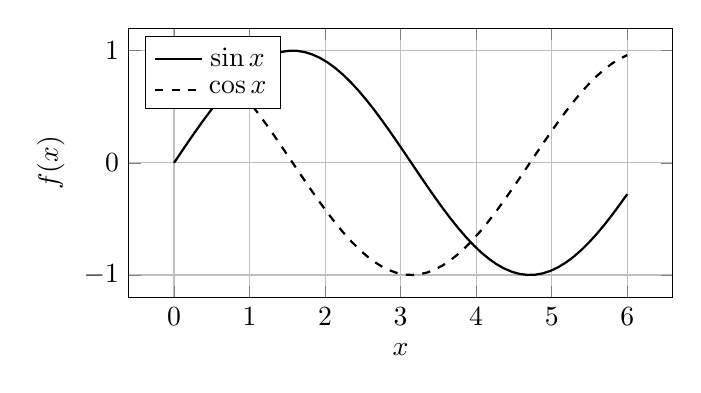
\begin{tikzpicture}
    \begin{axis}[
        width=0.7\linewidth, height=5cm,
        xlabel={$x$}, ylabel={$f(x)$},
        legend pos=north west, grid=both,
      ]
      \addplot[domain=0:6, samples=60, thick] {sin(deg(x))};
      \addlegendentry{$\sin x$}
      \addplot[domain=0:6, samples=60, thick, dashed] {cos(deg(x))};
      \addlegendentry{$\cos x$}
    \end{axis}
  \end{tikzpicture}
  \caption{\fixme{A plot produced with \textsf{pgfplots}.}}
  \label{fig:example-plot}
\end{figure}

% --------------------------------------------------------------------------
\section{Tables}
\label{sec:example-tables}

Table~\ref{tab:example} is a \textsf{tabularray} table with \textsf{booktabs} rules.

\begin{table}[htbp]
  \centering
  \caption{\fixme{Example table caption.}}
  \label{tab:example}
  \begin{tblr}{colspec={lcc}, row{1}={font=\bfseries}}
    \toprule
    Quantity & Symbol & Value \\
    \midrule
    Density        & $\rho$ & \num{7800} \\
    Dynamic viscosity & $\mu$  & \num{6e-3} \\
    Surface tension   & $\sigma$ & \num{1.8} \\
    \bottomrule
  \end{tblr}
\end{table}
